\documentclass[]{book}
\usepackage{lmodern}
\usepackage{amssymb,amsmath}
\usepackage{ifxetex,ifluatex}
\usepackage{fixltx2e} % provides \textsubscript
\ifnum 0\ifxetex 1\fi\ifluatex 1\fi=0 % if pdftex
  \usepackage[T1]{fontenc}
  \usepackage[utf8]{inputenc}
\else % if luatex or xelatex
  \ifxetex
    \usepackage{mathspec}
  \else
    \usepackage{fontspec}
  \fi
  \defaultfontfeatures{Ligatures=TeX,Scale=MatchLowercase}
\fi
% use upquote if available, for straight quotes in verbatim environments
\IfFileExists{upquote.sty}{\usepackage{upquote}}{}
% use microtype if available
\IfFileExists{microtype.sty}{%
\usepackage{microtype}
\UseMicrotypeSet[protrusion]{basicmath} % disable protrusion for tt fonts
}{}
\usepackage[margin=1in]{geometry}
\usepackage{hyperref}
\hypersetup{unicode=true,
            pdftitle={Do not use averages with Likert scale data},
            pdfauthor={Dwight Barry},
            pdfborder={0 0 0},
            breaklinks=true}
\urlstyle{same}  % don't use monospace font for urls
\usepackage{natbib}
\bibliographystyle{plainnat}
\usepackage{color}
\usepackage{fancyvrb}
\newcommand{\VerbBar}{|}
\newcommand{\VERB}{\Verb[commandchars=\\\{\}]}
\DefineVerbatimEnvironment{Highlighting}{Verbatim}{commandchars=\\\{\}}
% Add ',fontsize=\small' for more characters per line
\usepackage{framed}
\definecolor{shadecolor}{RGB}{248,248,248}
\newenvironment{Shaded}{\begin{snugshade}}{\end{snugshade}}
\newcommand{\KeywordTok}[1]{\textcolor[rgb]{0.13,0.29,0.53}{\textbf{{#1}}}}
\newcommand{\DataTypeTok}[1]{\textcolor[rgb]{0.13,0.29,0.53}{{#1}}}
\newcommand{\DecValTok}[1]{\textcolor[rgb]{0.00,0.00,0.81}{{#1}}}
\newcommand{\BaseNTok}[1]{\textcolor[rgb]{0.00,0.00,0.81}{{#1}}}
\newcommand{\FloatTok}[1]{\textcolor[rgb]{0.00,0.00,0.81}{{#1}}}
\newcommand{\ConstantTok}[1]{\textcolor[rgb]{0.00,0.00,0.00}{{#1}}}
\newcommand{\CharTok}[1]{\textcolor[rgb]{0.31,0.60,0.02}{{#1}}}
\newcommand{\SpecialCharTok}[1]{\textcolor[rgb]{0.00,0.00,0.00}{{#1}}}
\newcommand{\StringTok}[1]{\textcolor[rgb]{0.31,0.60,0.02}{{#1}}}
\newcommand{\VerbatimStringTok}[1]{\textcolor[rgb]{0.31,0.60,0.02}{{#1}}}
\newcommand{\SpecialStringTok}[1]{\textcolor[rgb]{0.31,0.60,0.02}{{#1}}}
\newcommand{\ImportTok}[1]{{#1}}
\newcommand{\CommentTok}[1]{\textcolor[rgb]{0.56,0.35,0.01}{\textit{{#1}}}}
\newcommand{\DocumentationTok}[1]{\textcolor[rgb]{0.56,0.35,0.01}{\textbf{\textit{{#1}}}}}
\newcommand{\AnnotationTok}[1]{\textcolor[rgb]{0.56,0.35,0.01}{\textbf{\textit{{#1}}}}}
\newcommand{\CommentVarTok}[1]{\textcolor[rgb]{0.56,0.35,0.01}{\textbf{\textit{{#1}}}}}
\newcommand{\OtherTok}[1]{\textcolor[rgb]{0.56,0.35,0.01}{{#1}}}
\newcommand{\FunctionTok}[1]{\textcolor[rgb]{0.00,0.00,0.00}{{#1}}}
\newcommand{\VariableTok}[1]{\textcolor[rgb]{0.00,0.00,0.00}{{#1}}}
\newcommand{\ControlFlowTok}[1]{\textcolor[rgb]{0.13,0.29,0.53}{\textbf{{#1}}}}
\newcommand{\OperatorTok}[1]{\textcolor[rgb]{0.81,0.36,0.00}{\textbf{{#1}}}}
\newcommand{\BuiltInTok}[1]{{#1}}
\newcommand{\ExtensionTok}[1]{{#1}}
\newcommand{\PreprocessorTok}[1]{\textcolor[rgb]{0.56,0.35,0.01}{\textit{{#1}}}}
\newcommand{\AttributeTok}[1]{\textcolor[rgb]{0.77,0.63,0.00}{{#1}}}
\newcommand{\RegionMarkerTok}[1]{{#1}}
\newcommand{\InformationTok}[1]{\textcolor[rgb]{0.56,0.35,0.01}{\textbf{\textit{{#1}}}}}
\newcommand{\WarningTok}[1]{\textcolor[rgb]{0.56,0.35,0.01}{\textbf{\textit{{#1}}}}}
\newcommand{\AlertTok}[1]{\textcolor[rgb]{0.94,0.16,0.16}{{#1}}}
\newcommand{\ErrorTok}[1]{\textcolor[rgb]{0.64,0.00,0.00}{\textbf{{#1}}}}
\newcommand{\NormalTok}[1]{{#1}}
\usepackage{longtable,booktabs}
\usepackage{graphicx,grffile}
\makeatletter
\def\maxwidth{\ifdim\Gin@nat@width>\linewidth\linewidth\else\Gin@nat@width\fi}
\def\maxheight{\ifdim\Gin@nat@height>\textheight\textheight\else\Gin@nat@height\fi}
\makeatother
% Scale images if necessary, so that they will not overflow the page
% margins by default, and it is still possible to overwrite the defaults
% using explicit options in \includegraphics[width, height, ...]{}
\setkeys{Gin}{width=\maxwidth,height=\maxheight,keepaspectratio}
\IfFileExists{parskip.sty}{%
\usepackage{parskip}
}{% else
\setlength{\parindent}{0pt}
\setlength{\parskip}{6pt plus 2pt minus 1pt}
}
\setlength{\emergencystretch}{3em}  % prevent overfull lines
\providecommand{\tightlist}{%
  \setlength{\itemsep}{0pt}\setlength{\parskip}{0pt}}
\setcounter{secnumdepth}{5}
% Redefines (sub)paragraphs to behave more like sections
\ifx\paragraph\undefined\else
\let\oldparagraph\paragraph
\renewcommand{\paragraph}[1]{\oldparagraph{#1}\mbox{}}
\fi
\ifx\subparagraph\undefined\else
\let\oldsubparagraph\subparagraph
\renewcommand{\subparagraph}[1]{\oldsubparagraph{#1}\mbox{}}
\fi

%%% Use protect on footnotes to avoid problems with footnotes in titles
\let\rmarkdownfootnote\footnote%
\def\footnote{\protect\rmarkdownfootnote}

%%% Change title format to be more compact
\usepackage{titling}

% Create subtitle command for use in maketitle
\newcommand{\subtitle}[1]{
  \posttitle{
    \begin{center}\large#1\end{center}
    }
}

\setlength{\droptitle}{-2em}
  \title{Do not use averages with Likert scale data}
  \pretitle{\vspace{\droptitle}\centering\huge}
  \posttitle{\par}
  \author{Dwight Barry}
  \preauthor{\centering\large\emph}
  \postauthor{\par}
  \predate{\centering\large\emph}
  \postdate{\par}
  \date{2017-01-04}

\usepackage{booktabs}

\begin{document}
\maketitle

{
\setcounter{tocdepth}{1}
\tableofcontents
}
\chapter*{About}\label{about}
\addcontentsline{toc}{chapter}{About}

\begin{center}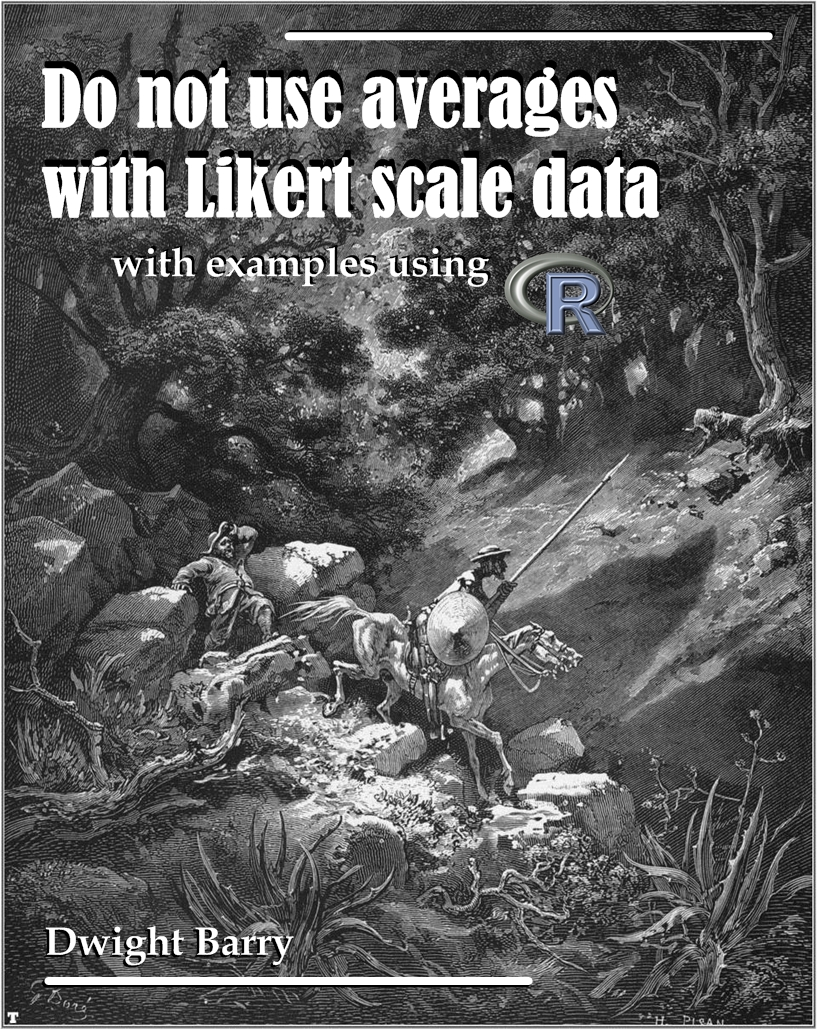
\includegraphics[width=11.35in]{images/likert_cover} \end{center}

This is a short overview of why averages don't work well for evaluating
Likert scale or other ordinal-scale data, and what to do instead, with
examples using R. While the examples are focused on healthcare surveys,
the lessons apply to any use of ordinal scale data.

Note: all of the data in this document is fake, created specifically to
illustrate particular points.

\emph{Contact/Twitter:} \citet{healthstatsdude}

\emph{PDF version:}

\emph{Website:} \url{https://bookdown.org/Rmadillo/likert/}

\emph{Corrections/Pull requests:}
\url{https://github.com/Rmadillo/likert}

\emph{Cover image}: Gustave Doré, 1863. Illustration 12 for Cervantes's
\emph{Don Quixote}.
\href{https://commons.wikimedia.org/w/index.php?curid=677913}{Public
Domain}.


\includegraphics[width=1.22in]{images/cc-by-sa}

\emph{This work is licensed under a
\href{https://creativecommons.org/licenses/by-sa/4.0/}{Creative Commons
Attribution-ShareAlike 4.0 License}.}

\section*{R packgaes}\label{r-packgaes}
\addcontentsline{toc}{section}{R packgaes}

\begin{Shaded}
\begin{Highlighting}[]
\NormalTok{#### Packages ####}
\KeywordTok{library}\NormalTok{(grid)}
\KeywordTok{library}\NormalTok{(nnet)}
\KeywordTok{library}\NormalTok{(coin)}
\KeywordTok{library}\NormalTok{(boot)}
\KeywordTok{library}\NormalTok{(simpleboot)}
\KeywordTok{library}\NormalTok{(knitr)}
\KeywordTok{library}\NormalTok{(ggplot2)}
\KeywordTok{library}\NormalTok{(dplyr)}
\KeywordTok{library}\NormalTok{(AICcmodavg)}
\KeywordTok{library}\NormalTok{(polycor)}
\KeywordTok{library}\NormalTok{(likert)}
\KeywordTok{library}\NormalTok{(MASS)}
\KeywordTok{library}\NormalTok{(ordinal)}
\end{Highlighting}
\end{Shaded}

\section*{Data}\label{data}
\addcontentsline{toc}{section}{Data}

\begin{Shaded}
\begin{Highlighting}[]
\NormalTok{#### Basic example data set ####}
\NormalTok{person =}\StringTok{ }\KeywordTok{c}\NormalTok{(}\StringTok{'A'}\NormalTok{,}\StringTok{'B'}\NormalTok{,}\StringTok{'C'}\NormalTok{,}\StringTok{'D'}\NormalTok{,}\StringTok{'E'}\NormalTok{,}\StringTok{'F'}\NormalTok{)}

\CommentTok{# Original }
\NormalTok{year1 =}\StringTok{ }\KeywordTok{c}\NormalTok{(}\DecValTok{5}\NormalTok{,}\DecValTok{4}\NormalTok{,}\DecValTok{4}\NormalTok{,}\DecValTok{4}\NormalTok{,}\DecValTok{4}\NormalTok{,}\DecValTok{4}\NormalTok{)}
\NormalTok{year2 =}\StringTok{ }\KeywordTok{c}\NormalTok{(}\DecValTok{2}\NormalTok{,}\DecValTok{5}\NormalTok{,}\DecValTok{5}\NormalTok{,}\DecValTok{5}\NormalTok{,}\DecValTok{5}\NormalTok{,}\DecValTok{4}\NormalTok{)}
\NormalTok{year3 =}\StringTok{ }\KeywordTok{c}\NormalTok{(}\DecValTok{3}\NormalTok{,}\DecValTok{5}\NormalTok{,}\DecValTok{5}\NormalTok{,}\DecValTok{5}\NormalTok{,}\DecValTok{5}\NormalTok{,}\DecValTok{3}\NormalTok{)}
\NormalTok{year4 =}\StringTok{ }\KeywordTok{c}\NormalTok{(}\DecValTok{1}\NormalTok{,}\DecValTok{5}\NormalTok{,}\DecValTok{5}\NormalTok{,}\DecValTok{5}\NormalTok{,}\DecValTok{5}\NormalTok{,}\DecValTok{5}\NormalTok{)}

\CommentTok{# A more obvious version}
\CommentTok{# year1 = c(3,3,3,3,3,3)}
\CommentTok{# year2 = c(4,4,4,2,2,2)}
\CommentTok{# year3 = c(5,4,3,3,2,1)}
\CommentTok{# year4 = c(5,5,5,1,1,1)}
 
\NormalTok{ex_1 =}\StringTok{ }\KeywordTok{data.frame}\NormalTok{(person, year1, year2, year3, year4)}
 
\NormalTok{ex_1_long =}\StringTok{ }\NormalTok{reshape2::}\KeywordTok{melt}\NormalTok{(ex_1)}

\NormalTok{#### Larger example data set ####}

\KeywordTok{set.seed}\NormalTok{(}\DecValTok{29}\NormalTok{)}

\NormalTok{md =}\StringTok{ }\KeywordTok{data.frame}\NormalTok{(}\DataTypeTok{Group =} \KeywordTok{as.character}\NormalTok{(}\StringTok{"MD"}\NormalTok{), }
    \DataTypeTok{Response1 =} \KeywordTok{ordered}\NormalTok{(}\KeywordTok{sample}\NormalTok{(}\DecValTok{1}\NormalTok{:}\DecValTok{5}\NormalTok{, }\DecValTok{100}\NormalTok{, }\DataTypeTok{replace=}\NormalTok{T, }\DataTypeTok{prob=}\KeywordTok{c}\NormalTok{(.}\DecValTok{1}\NormalTok{,.}\DecValTok{1}\NormalTok{,.}\DecValTok{1}\NormalTok{,.}\DecValTok{2}\NormalTok{,.}\DecValTok{5}\NormalTok{))), }
    \DataTypeTok{Response2 =} \KeywordTok{ordered}\NormalTok{(}\KeywordTok{sample}\NormalTok{(}\DecValTok{1}\NormalTok{:}\DecValTok{5}\NormalTok{, }\DecValTok{100}\NormalTok{, }\DataTypeTok{replace=}\NormalTok{T, }\DataTypeTok{prob=}\KeywordTok{c}\NormalTok{(.}\DecValTok{1}\NormalTok{,.}\DecValTok{3}\NormalTok{,.}\DecValTok{3}\NormalTok{,.}\DecValTok{25}\NormalTok{,.}\DecValTok{15}\NormalTok{))))}
\NormalTok{rn =}\StringTok{ }\KeywordTok{data.frame}\NormalTok{(}\DataTypeTok{Group =} \KeywordTok{as.character}\NormalTok{(}\StringTok{"RN"}\NormalTok{), }
    \DataTypeTok{Response1 =} \KeywordTok{ordered}\NormalTok{(}\KeywordTok{sample}\NormalTok{(}\DecValTok{1}\NormalTok{:}\DecValTok{5}\NormalTok{, }\DecValTok{100}\NormalTok{, }\DataTypeTok{replace=}\NormalTok{T, }\DataTypeTok{prob=}\KeywordTok{c}\NormalTok{(.}\DecValTok{1}\NormalTok{,.}\DecValTok{1}\NormalTok{,.}\DecValTok{5}\NormalTok{,.}\DecValTok{2}\NormalTok{,.}\DecValTok{1}\NormalTok{))), }
    \DataTypeTok{Response2 =} \KeywordTok{ordered}\NormalTok{(}\KeywordTok{sample}\NormalTok{(}\DecValTok{1}\NormalTok{:}\DecValTok{5}\NormalTok{, }\DecValTok{100}\NormalTok{, }\DataTypeTok{replace=}\NormalTok{T, }\DataTypeTok{prob=}\KeywordTok{c}\NormalTok{(.}\DecValTok{1}\NormalTok{,.}\DecValTok{15}\NormalTok{,.}\DecValTok{45}\NormalTok{,.}\DecValTok{15}\NormalTok{,.}\DecValTok{15}\NormalTok{))))}
 
\NormalTok{both =}\StringTok{ }\KeywordTok{rbind}\NormalTok{(md, rn)}

\CommentTok{# Add some NAs }
\NormalTok{make_NAs =}\StringTok{ }\KeywordTok{sample}\NormalTok{(}\DecValTok{1}\NormalTok{:}\DecValTok{200}\NormalTok{, }\DecValTok{15}\NormalTok{, }\DataTypeTok{replace=}\NormalTok{F)}
\NormalTok{both$Response1[make_NAs] =}\StringTok{ }\OtherTok{NA}
 
\NormalTok{make_NAs2 =}\StringTok{ }\KeywordTok{sample}\NormalTok{(}\DecValTok{1}\NormalTok{:}\DecValTok{200}\NormalTok{, }\DecValTok{15}\NormalTok{, }\DataTypeTok{replace=}\NormalTok{F)}
\NormalTok{both$Response2[make_NAs2] =}\StringTok{ }\OtherTok{NA}

\CommentTok{# Add question names to data}
\KeywordTok{names}\NormalTok{(both) =}\StringTok{ }\KeywordTok{c}\NormalTok{(}\StringTok{"EmployeeType"}\NormalTok{, }
                \StringTok{"My team works well together."}\NormalTok{, }
                \StringTok{"I have the tools I need to do my job."}\NormalTok{)}

\NormalTok{#### Dashboarding pain scores example ####}

\CommentTok{# Create list for random pain scores}
\NormalTok{pain_list =}\StringTok{ }\KeywordTok{list}\NormalTok{()}

\NormalTok{for(i in }\DecValTok{1}\NormalTok{:}\DecValTok{24}\NormalTok{)\{}
  \KeywordTok{set.seed}\NormalTok{(i)}
  \NormalTok{pain_level =}\StringTok{ }\KeywordTok{ordered}\NormalTok{(}\KeywordTok{sample}\NormalTok{(}\KeywordTok{c}\NormalTok{(}\StringTok{"Low"}\NormalTok{, }\StringTok{"Medium"}\NormalTok{, }\StringTok{"High"}\NormalTok{), }\DataTypeTok{size =} \KeywordTok{sample}\NormalTok{(}\DecValTok{10}\NormalTok{:}\DecValTok{30}\NormalTok{),}
    \DataTypeTok{replace =} \NormalTok{T, }\DataTypeTok{prob =} \KeywordTok{c}\NormalTok{(.}\DecValTok{15}\NormalTok{, .}\DecValTok{45}\NormalTok{, .}\DecValTok{40}\NormalTok{)), }\DataTypeTok{levels =} \KeywordTok{c}\NormalTok{(}\StringTok{"Low"}\NormalTok{, }\StringTok{"Medium"}\NormalTok{, }\StringTok{"High"}\NormalTok{))}
  \NormalTok{pain_list[[i]] =}\StringTok{ }\KeywordTok{table}\NormalTok{(pain_level)}
\NormalTok{\}}

\CommentTok{# Unlist into a data frame}
\NormalTok{pain_df =}\StringTok{ }\KeywordTok{data.frame}\NormalTok{(}\KeywordTok{matrix}\NormalTok{(}\KeywordTok{unlist}\NormalTok{(pain_list), }\DataTypeTok{nrow=}\DecValTok{24}\NormalTok{, }\DataTypeTok{byrow=}\NormalTok{T))}
\KeywordTok{colnames}\NormalTok{(pain_df) =}\StringTok{ }\KeywordTok{c}\NormalTok{(}\StringTok{"Low"}\NormalTok{, }\StringTok{"Medium"}\NormalTok{, }\StringTok{"High"}\NormalTok{)}

\CommentTok{# Add some months}
\NormalTok{pain_scores =}\StringTok{ }\KeywordTok{data.frame}\NormalTok{(}\DataTypeTok{Month =} \KeywordTok{seq}\NormalTok{(}\KeywordTok{as.Date}\NormalTok{(}\StringTok{"2014-10-01"}\NormalTok{), }\DataTypeTok{by =} \StringTok{"month"}\NormalTok{, }
  \DataTypeTok{length.out =} \DecValTok{24}\NormalTok{), pain_df)}

\CommentTok{# Melt into long form, I really should learn tidyr}
\NormalTok{pain_scores =}\StringTok{ }\NormalTok{reshape2::}\KeywordTok{melt}\NormalTok{(pain_scores, }\DataTypeTok{id.vars =} \StringTok{"Month"}\NormalTok{, }
  \DataTypeTok{variable.name =} \StringTok{"Pain_Group"}\NormalTok{, }\DataTypeTok{value.name =} \StringTok{"Count"}\NormalTok{)}

\CommentTok{# Summarize to get counts and percentages}
\NormalTok{surgeries_pain =}\StringTok{ }\NormalTok{pain_scores %>%}\StringTok{ }
\StringTok{  }\KeywordTok{group_by}\NormalTok{(Month) %>%}
\StringTok{  }\KeywordTok{mutate}\NormalTok{(}\DataTypeTok{Surgeries =} \KeywordTok{sum}\NormalTok{(Count), }\DataTypeTok{percent =} \NormalTok{(Count /}\StringTok{ }\KeywordTok{sum}\NormalTok{(Count)), }
    \DataTypeTok{cumsum =} \KeywordTok{cumsum}\NormalTok{(percent))}

\NormalTok{#### For use with chi-square and regression models ####}

\CommentTok{# Get rid of NAs}
\NormalTok{both2 =}\StringTok{ }\KeywordTok{na.omit}\NormalTok{(both)}

\CommentTok{# Rename columns to something more R-friendly}
\KeywordTok{names}\NormalTok{(both2) =}\StringTok{ }\KeywordTok{c}\NormalTok{(}\StringTok{"EmployeeType"}\NormalTok{, }\StringTok{"Teamwork"}\NormalTok{, }\StringTok{"Tools"}\NormalTok{)}

\CommentTok{# Reverse the levels so 5 will be at top of mosaic plot}
\NormalTok{both2$Teamwork =}\StringTok{ }\KeywordTok{ordered}\NormalTok{(both2$Teamwork, }\DataTypeTok{levels =} \KeywordTok{c}\NormalTok{(}\StringTok{"5"}\NormalTok{, }\StringTok{"4"}\NormalTok{, }\StringTok{"3"}\NormalTok{, }\StringTok{"2"}\NormalTok{, }\StringTok{"1"}\NormalTok{))}

\CommentTok{# Make a table object}
\NormalTok{both2_tab =}\StringTok{ }\KeywordTok{xtabs}\NormalTok{(~}\StringTok{ }\NormalTok{both2$EmployeeType +}\StringTok{ }\NormalTok{both2$Teamwork)}

\CommentTok{# For multinomial and prop odds models}
\NormalTok{both3 =}\StringTok{ }\NormalTok{both2}

\CommentTok{# Bring axis back to normal}
\NormalTok{both3$Teamwork =}\StringTok{ }\KeywordTok{ordered}\NormalTok{(both3$Teamwork, }\DataTypeTok{levels =} \KeywordTok{c}\NormalTok{(}\StringTok{"1"}\NormalTok{, }\StringTok{"2"}\NormalTok{, }\StringTok{"3"}\NormalTok{, }\StringTok{"4"}\NormalTok{, }\StringTok{"5"}\NormalTok{))}

\CommentTok{# Data frame for proportional odds regression}
\NormalTok{Teamwork_tab_long =}\StringTok{ }\NormalTok{both3[,}\DecValTok{1}\NormalTok{:}\DecValTok{2}\NormalTok{] %>%}
\StringTok{  }\KeywordTok{group_by}\NormalTok{(EmployeeType, Teamwork) %>%}
\StringTok{  }\KeywordTok{summarize}\NormalTok{(}\DataTypeTok{Count =} \KeywordTok{n}\NormalTok{())}

\CommentTok{# Function to turn counts into rows I found laying around the web somewhere}
\NormalTok{countsToCases =}\StringTok{ }\NormalTok{function(x, }\DataTypeTok{countcol =} \StringTok{"Count"}\NormalTok{) \{}
    \CommentTok{# Get the row indices to pull from x}
    \NormalTok{idx =}\StringTok{ }\KeywordTok{rep.int}\NormalTok{(}\KeywordTok{seq_len}\NormalTok{(}\KeywordTok{nrow}\NormalTok{(x)), x[[countcol]])}
    \CommentTok{# Drop count column}
    \NormalTok{x[[countcol]] =}\StringTok{ }\OtherTok{NULL}
    \CommentTok{# Get the rows from x}
    \NormalTok{x[idx, ]}
\NormalTok{\}}

\CommentTok{# Make a data frame for prop odds}
\NormalTok{Teamwork_tab_long$Teamwork_Group =}\StringTok{ }\KeywordTok{as.numeric}\NormalTok{(Teamwork_tab_long$Teamwork) }
\NormalTok{Teamwork_tab_long$Teamwork =}\StringTok{ }\KeywordTok{ordered}\NormalTok{(Teamwork_tab_long$Teamwork) }
\NormalTok{tab_df =}\StringTok{ }\KeywordTok{data.frame}\NormalTok{(}\KeywordTok{countsToCases}\NormalTok{(Teamwork_tab_long, }\DataTypeTok{countcol=}\StringTok{"Count"}\NormalTok{))}
\end{Highlighting}
\end{Shaded}

\chapter{Summary}\label{summary}

\chapter{\texorpdfstring{\emph{Why not?} A simple
example}{Why not? A simple example}}\label{why-not-a-simple-example}

\chapter{\texorpdfstring{\emph{Always}
visualize}{Always visualize}}\label{always-visualize}

\chapter{\texorpdfstring{\emph{Neutral} scores
matter}{Neutral scores matter}}\label{neutral-scores-matter}

\chapter{How many respondents are
enough?}\label{how-many-respondents-are-enough}

\chapter{\texorpdfstring{Is there a \emph{significant}
difference?}{Is there a significant difference?}}\label{is-there-a-significant-difference}

\chapter{A final word}\label{a-final-word}

\chapter*{Appendix: Measurement Levels \& Summary
Statistics}\label{appendix-measurement-levels-summary-statistics}
\addcontentsline{toc}{chapter}{Appendix: Measurement Levels \& Summary
Statistics}


\end{document}
